% -*- latex -*-
%%%%%%%%%%%%%%%%%%%%%%%%%%%%%%%%%%%%%%%%%%%%%%%%%%%%%%%%%%%%%%%%
%%%%%%%%%%%%%%%%%%%%%%%%%%%%%%%%%%%%%%%%%%%%%%%%%%%%%%%%%%%%%%%%
%%%%
%%%% This text file is part of the source of 
%%%% `Parallel Computing'
%%%% by Victor Eijkhout, copyright 2012-6
%%%%
%%%% grid.tex : programming project for grid PDE operations
%%%%
%%%%%%%%%%%%%%%%%%%%%%%%%%%%%%%%%%%%%%%%%%%%%%%%%%%%%%%%%%%%%%%%
%%%%%%%%%%%%%%%%%%%%%%%%%%%%%%%%%%%%%%%%%%%%%%%%%%%%%%%%%%%%%%%%

In this section we will gradually build a semi-realistic example
program. To get you started some pieces have already been written:
as a starting point look at \n{code/mpi/c/grid.cxx}.

\Level 0 {Description of the problem}

With this example you will investigate several strategies for
implementing a simple iterative method. Let's say you have a
two-dimensional grid of datapoints $G=\{g_{ij}\colon 0\leq
i<n_i,\,0\leq j<n_j\}$ and you want to compute~$G'$ where
\begin{equation}
g'_{ij} = 1/4 \cdot (g_{i+1,j}+g_{i-1,j}+g_{i,j+1}+g_{i,j-1}).
\label{eq:grid-update}
\end{equation}

This is easy enough to implement sequentially, but in parallel this
requires some care.

Let's divide the grid $G$ and divide it over a two-dimension grid of
$p_i\times p_j$
processors. (Other strategies exist, but this one scales best; see
section~\HPSCref{sec:pspmvp}.)
Formally, we define two sequences of points
\[ 0=i_0<\cdots<i_{p_i}<i_{p_i+1}=n_i,\quad 
   0<j_0<\cdots<j_{p_j}<i_{p_j+1}=n_j
\]
and we say that processor $(p,q)$ computes $g_{ij}$ for
\[ i_p\leq i<i_{p+1}, \quad j_q\leq j<j_{q+1}.
\]
From formula~\eqref{eq:grid-update} you see that the processor then
needs one row of points on each side surrounding its part of the
grid. A~picture makes this clear; see figure~\ref{fig:ghost-grid}.
\begin{figure}
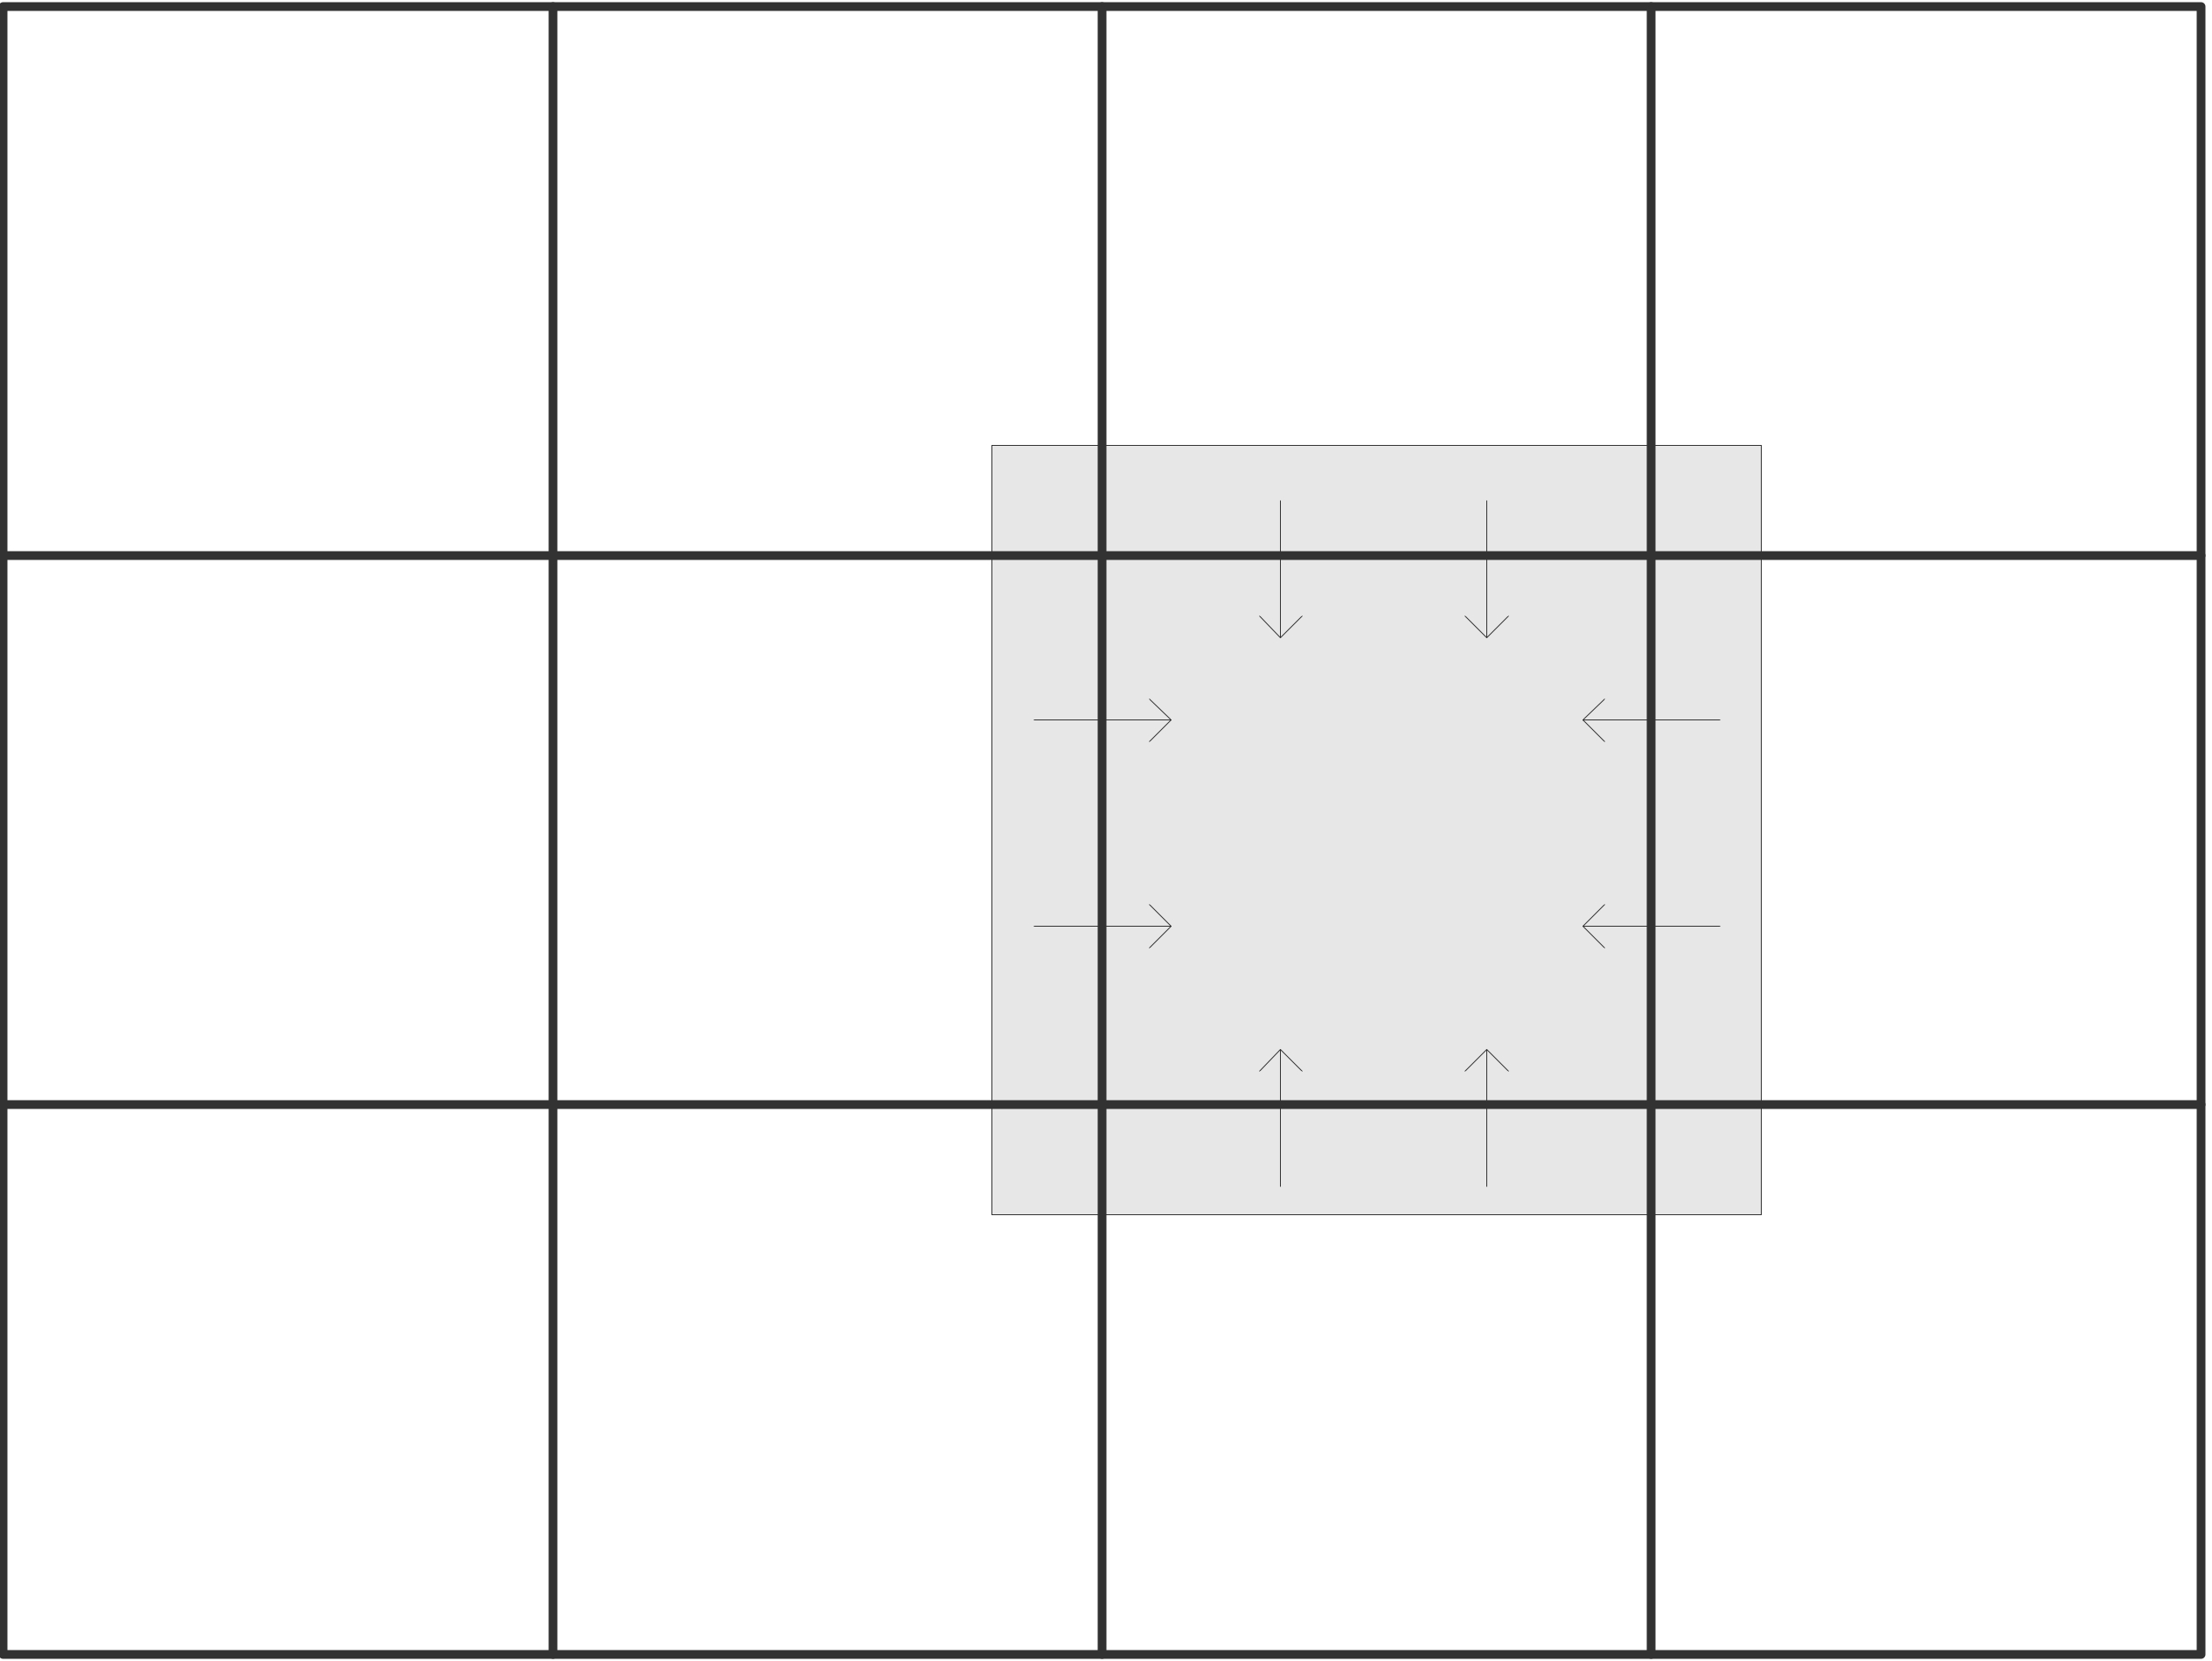
\includegraphics[scale=.1]{graphics/jacobi-average}
\caption{A grid divided over processors, with the `ghost' region indicated}
\label{fig:ghost-grid}
\end{figure}
These elements surrounding the processor's own part are called
the \indexterm{halo} or \indexterm{ghost region} of that processor.

The problem is now that the elements in the halo are stored on a
different processor, so communication is needed to gather them. In the
upcoming exercises you will have to use different strategies for doing
so.

\Level 0 {Code basics}

The program needs to read the values of the grid size and the
processor grid size from the commandline, as well as the number of
iterations. This routine does some error checking: if the number of
processors does not add up to the size of \n{MPI_COMM_WORLD}, a
nonzero error code is returned.
\begin{verbatim}
ierr = parameters_from_commandline
  (argc,argv,comm,&ni,&nj,&pi,&pj,&nit);
if (ierr) return MPI_Abort(comm,1);
\end{verbatim}
From the processor parameters we make a processor grid object:
\begin{verbatim}
processor_grid *pgrid = new processor_grid(comm,pi,pj);
\end{verbatim}
and from the numerical parameters we make a number grid:
\begin{verbatim}
number_grid *grid = new number_grid(pgrid,ni,nj);
\end{verbatim}
Number grids have a number of methods defined. To set the value of all
the elements belonging to a processor to that processor's number:
\begin{verbatim}
grid->set_test_values();
\end{verbatim}
To set random values:
\begin{verbatim}
grid->set_random_values();
\end{verbatim}
If you want to visualize the whole grid, the following call gathers
all values on processor zero and prints them:
\begin{verbatim}
grid->gather_and_print();
\end{verbatim}

Next we need to look at some data structure details.

The definition of the \n{number_grid} object starts as follows:
\begin{verbatim}
class number_grid {
public:
  processor_grid *pgrid;
  double *values,*shadow;
\end{verbatim}
where \n{values} contains the elements owned by the processor,
and \n{shadow} is intended to contain the values plus the ghost
region. So how does \n{shadow} receive those values? Well, the call looks 
like
\begin{verbatim}
grid->build_shadow();
\end{verbatim}
and you will need to supply the implementation of that.
Once you've done so, there is a routine that prints out the shadow array 
of each processor
\begin{verbatim}
grid->print_shadow();
\end{verbatim}
This routine does the sequenced printing that you implemented in
exercise~\ref{ex:hello-world-zero}.

In the file \n{code/mpi/c/grid_impl.cxx} you can see several uses of
the macro \n{INDEX}. This translates from a two-dimensional coordinate
system to one-dimensional. Its main use is letting you use $(i,j)$
coordinates for indexing the processor grid and the number grid: for
processors you need the translation to the linear rank, and for the
grid you need the translation to the linear array that holds the
values.

A good example of the use of \n{INDEX} is in the
\n{number_grid::relax} routine: this takes points from the \n{shadow}
array and averages them into a point of the \n{values} array. (To
understand the reason for this particular averaging,
see~\HPSCref{sec:2dbvp} and~\HPSCref{sec:jacobi-seidel}.) Note how the
\n{INDEX} macro is used to index in a
$\n{ilength}\times\n{jlength}$ target array \n{values}, while
reading from a $(\n{ilength}+2)\times(\n{jlength}+2)$ source array
\n{shadow}.
\begin{verbatim}
for (i=0; i<ilength; i++) {
  for (j=0; j<jlength; j++) {
    int c=0;
    double new_value=0.;
    for (c=0; c<5; c++) {
	int ioff=i+1+ioffsets[c],joff=j+1+joffsets[c];
	new_value += coefficients[c] * 
	  shadow[ INDEX(ioff,joff,ilength+2,jlength+2) ];
    }
    values[ INDEX(i,j,ilength,jlength) ] = new_value/8.;
  }
}
\end{verbatim}

